\documentclass[12pt]{article}


\usepackage{geometry}
 \geometry{
 a4paper,
 left=20mm,
 right=20mm,
 top=10mm	
 }

\usepackage{amssymb}
\usepackage[utf8]{inputenc}
\usepackage{graphicx}
\usepackage{amstext}
\usepackage{amsmath}


\newtheorem{theorem}{Definice}


\title{BI-ZNS - Neurčitost ve znalostních systémech, její vyjadřování a zpracování.}
\author{Vastl Martin}

\begin{document}
\maketitle
\author

Z důvodu toho, že  poznatky, které získáváme ze složitých systémů, jsou neurčité a vágní nebo jsou nepřesně vyjádřeny, musíme tyto neurčitosti být schopni modelovat.

Příčiny neurčitosti můžou být z důvodu dat:
\begin{itemize}
\item chybějící nebo nerelevantní data
\item nedůvěryhodná data (chyba měření, nedůvěryhodný zdroj)
\item nepřesná nebo nekonzistentní reprezentace dat (např. kódování)
\end{itemize}
nebo z důvodu nejistých znalostí:

\begin{itemize}
\item Znalost nemusí být platná ve všech případech.
\item Znalost může obsahovat vágní pojmy.
\end{itemize}

\section{Vyjádření neurčitosti}
Neurčitost bývá obvykle vyjádřena za pomocí nějaké numerické hodnoty. Využívá se např. váhy, pravděpodobnosti, stupně důvěry a podobně, které většinou nabývají hodnot od 0 od 1 nebo od -1 do 1. Dost často se neurčitost reprezentuje za pomocí dvou čísel, která např. reprezentuje střední hodnotu a rozptyl.

Přístupy v znalostních systémech můžou být založené na ad-hoc metodách  jako jsou faktory jistoty nebo pseudobayesovských přístupech nebo na metodách založené na teoretických principech jako je teorie pravděpodobnosti, fuzzy množin nebo fuzzy míry. 

\subsection{Problémy při zpracování neurčitosti}
Mezi hlavní problémy při zpracování neurčitosti patří jak kombinovat neurčitá pravidla, jak kombinovat neurčitost předpokladu s neurčitostí pravidla jako celku a jak stanovit neurčitost závěru k němuž vede několik pravidel se svou mírou neurčitosti.

\section{Vyjádření pomocí trojhodnotové logiky}
Do klasické logiky 1 a 0 se přidá nová hodnota X, která značí hodnotu unknown. Příklad operací:
\begin{figure}[ht]
\centering
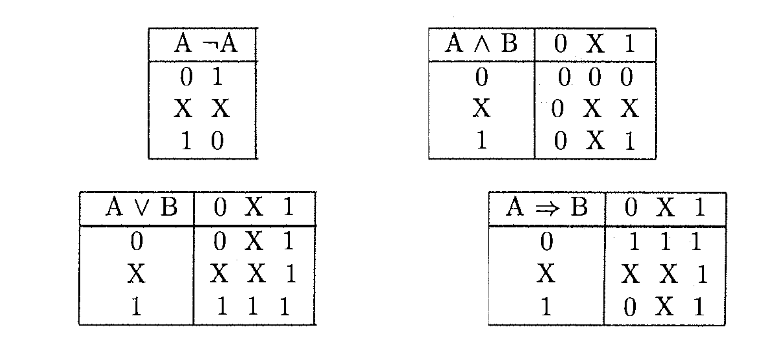
\includegraphics[width=0.5\linewidth]{logika}
\end{figure} 

\section{Vyjádření neurčitosti pomocí vah}
Využívá se algebraické teorie, kde jsou pravidla ve tvaru:
\begin{equation}
A\rightarrow B(w),
\end{equation}
kde $A$ (předpoklad pravidla) je pravidlo tvořené kombinací konjunkcí výroků a jejich negací, $B$ je závěr pravidla tvořen jedním výrokem a $w$ je váha pravidla a nabývá hodnot od -1 do 1, kde -1 znamená určitě ne, 0 nevím a 1 určitě ano.

\section{Bayesovský přístup ke zpracování neurčitosti}
Tento přístup je nejstarší a nejlépe definovanou technikou pro zpracování neurčitosti. Mějme pravidlo $E\rightarrow H$, která říká, že předpoklad $E$ podporuje závěr $H$, který lze vyjádřit za pomocí podmíněné pravdě\-podobnosti $P(H|E)$ a Bayseův vzorec pro výpočet podmíněné pravdě\-podobnosti je
\begin{equation}
P(H|E)=\frac{P(E|H)P(H)}{P(E)}.
\end{equation}

\subsection{Zpracování neurčitosti Šance}
Apriorní pravděpodobnostní šance je definována vztahem
\begin{equation}
O(H)=\frac{P(H)}{P(\lnot H)}=\frac{P(H)}{1-P(H)}
\end{equation}
Aposteriorní pravděpodobnostní šance je definována
\begin{equation}
O(H|E)=\frac{P(H|E)}{P(\lnot H|E)}
\end{equation}
a pravděpodobnost lze ze šance vypočítat podle $P=\frac{O}{O+1}$

\subsection{Míry postačitelnosti a nezbytnosti}
Z Bayesova vzorce pro aposteriorní pravděpodobnost plyne, že
\begin{equation}
O(H|E)=L\cdot O(H),
\end{equation}
kde $L=\frac{P(E|H)}{P(E|\lnot H)}$, která se nazývá míra postačitelnosti a velká hodnota $L\gg1$ říká, že předpoklad $E$ je postačující pro dokázání závěru $H$. Míru postačitelnosti $L$ zadává expert. Obdobně platí pro míru nezbytnosti $O(H|\lnot E)=\bar{L}\cdot O(H)$, kde $\bar{L}=\frac{P(\lnot E|H)}{P(\lnot E|\lnot H)}$ a malá hodnota $\bar{L}$ říká, že předpoklad $E$ je nezbytný pro dokázání závěru $H$.

\subsection{Váhy pravidel}
Pravidlo $E\rightarrow H(L)$ chápeme jako pravidlo \textit{if E then H with weight $L$ else H with weight $\bar{L}$}. Místo uvedených měr mohou být expertem zadány pravděpodobnosti $P(H|E)$ a $P(H|\lnot E)$ z nichž se tyto míry vypočtou
\begin{equation}
L=\frac{P(H|E)}{1-P(H|E)}\cdot \frac{1-P(H)}{P(H)}.
\end{equation}
Pokud bychom chtěli pravidla $E_1 \rightarrow H, E_2 \rightarrow H, \ldots, E_n \rightarrow H$ Pak aposteriorní šance při nezávislosti předpokladů $E_i$ se vypočte podle vztahu:
\begin{equation}
O(H|E_1 \wedge E_2 \wedge \ldots \wedge E_n)=L_1\cdot \ldots \cdot L_n \cdot O(H).
\end{equation}
Pokud místo přesných $E_i$ jsou k dispozici pouze pozorování $E'_i$, pak aposteriorní šance vypočte podle vztahu:
\begin{equation}
O(H|E'_1 \wedge E'_2 \wedge \ldots \wedge E'_n)=L'_1\cdot \ldots \cdot L'_n \cdot O(H),
\end{equation}
kde $L'_i=\frac{O(H|E'_i)}{O(H)}$. Pokud chceme předpoklady kombinovat můžeme využít vztahů z fuzzy logiky.
\begin{equation}
\begin{aligned}
P(E_1 \lor E_2) = \text{max}\{P(E_1), P(E_2)\}\\
P(E_1 \wedge E_2) = \text{min}\{P(E_1), P(E_2)\}
\end{aligned}
\end{equation}

\subsection{Výhody a nevýhody Bayesovských přístupů}
\subsubsection*{Výhody}
\begin{itemize}
\item Dobře podložené teoretické základy
\item Dobře definovaná sémantika rozhodování
\end{itemize}
\subsubsection*{Nevýhody}
\begin{itemize}
\item Potřeba stanovení velkého množství různých pravděpodobnostní
\item Riziko neúplnosti a/nebo nekonzistence dat
\item Předpoklady (evidence) $E$ i by měly být nezávislé, což v praxi často nebývá splněno
\item Riziko ztráty informace v důsledku popisu neurčitosti jedním číslem (ne\-přesnost vyjá\-dření)
\end{itemize}


\section{Přístup založený na faktorech jistoty}
Faktory jistoty (Certainty Factors) byly poprvé použity v systému MYCIN. Jejich cílem je eliminovat některé slabiny čistě pravděpodobnostního přístupu. Znalosti jsou vyjádřeny opět ve tvaru pravidel $E\rightarrow H$, přičemž za každým pravidlem je připojen faktor jistoty CF.

Faktor jistoty (CF) nabývá hodnot z intervalu $[–1,1]$, kde $1$ je absolutní důvěra a $-1$ absolutní nedůvěra a je určen spojením dílčích měr důvěry MB a nedůvěry MD do jednoho vztahu:
\begin{equation}
\text{CF}=\frac{MB-MD}{1-\min{\{MB, MD\}}},
\end{equation}
\begin{figure}[h!]
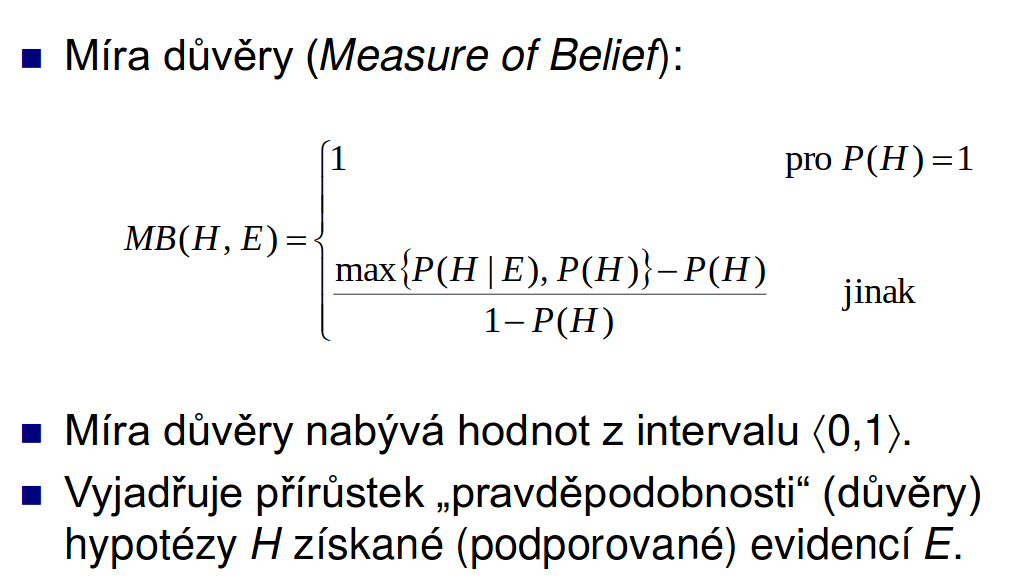
\includegraphics[scale=0.3]{duvera}
\end{figure}
\begin{figure}[h!]
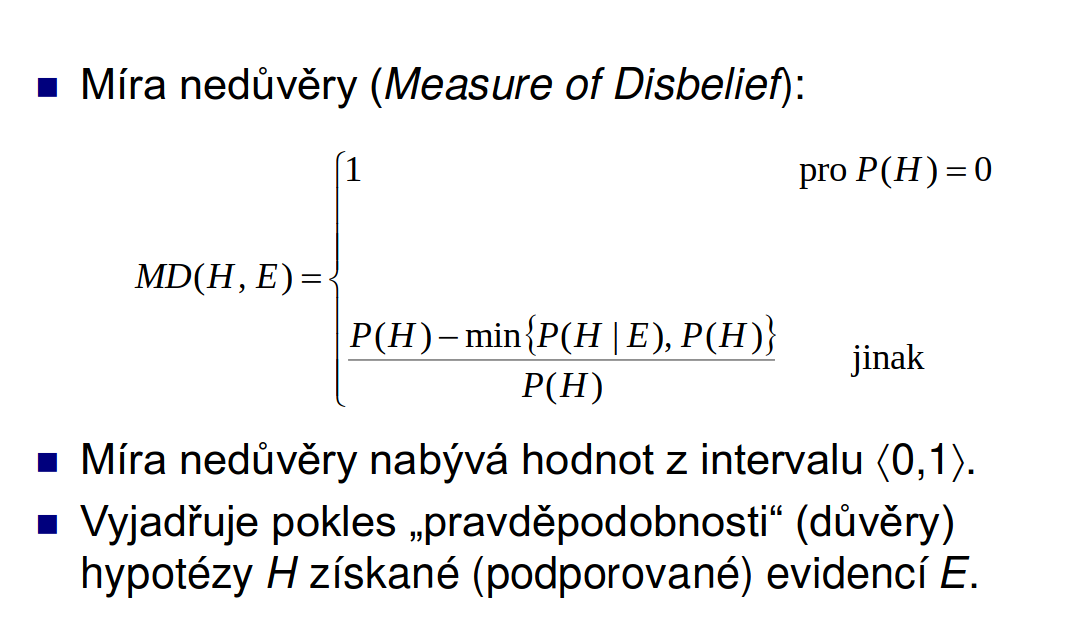
\includegraphics[scale=0.3]{neduvera}
\end{figure}
\begin{figure}[h!]
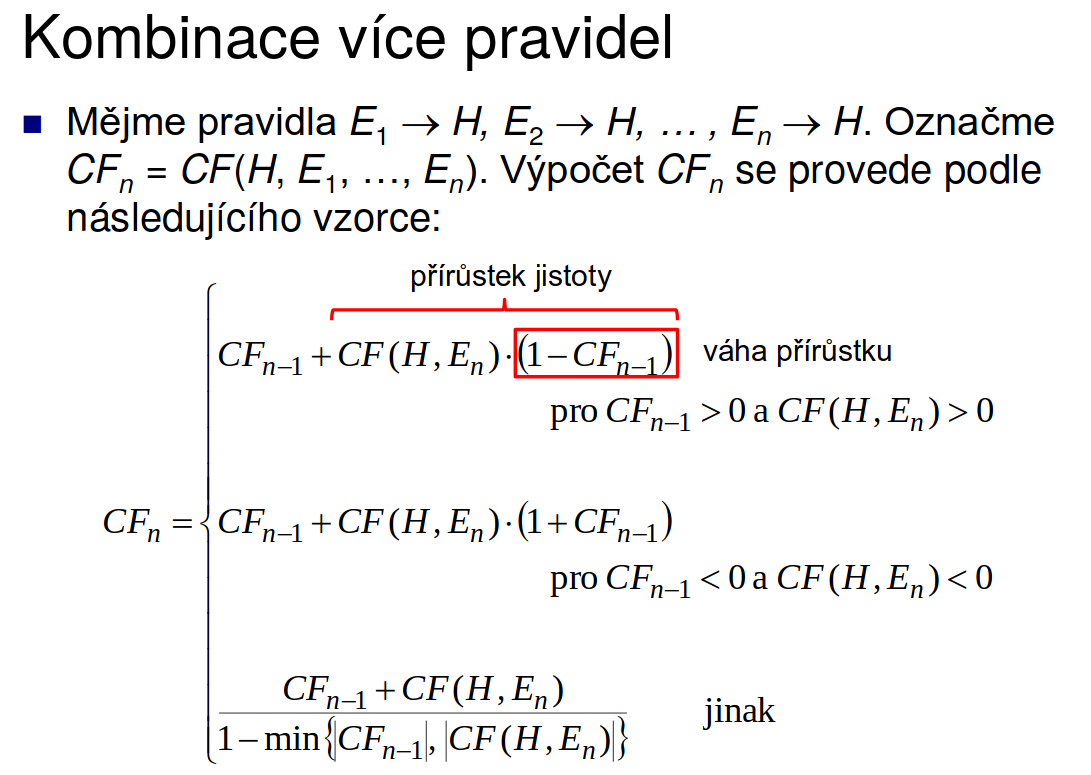
\includegraphics[scale=0.3]{kombinace}
\end{figure}


Pokud faktor jistoty není znám přesně nebo je zadán uživatelem, pak může být odvozen $CF_{NEW}(H, E)=CF_{OLD}(H, E)\cdot CF(E)$. Konjunkci a disjunkci předpokladů lze vypočítat jako v případě fuzzy množin:
\begin{equation}
\begin{aligned}
CF(E_1 \lor E_2) = \text{max}\{CF(E_1), CF(E_2)\}\\
CF(E_1 \wedge E_2) = \text{min}\{CF(E_1), CF(E_2)\}
\end{aligned}
\end{equation}



\subsection{Výhody a nevýhody faktorů jistoty}
\subsubsection*{Výhody}
\begin{itemize}
\item Jednoduchý a účinný výpočetní model
\item Sběr potřebných dat pro výpočty je podstatně snazší než u jiných metod.
\item Snazší implementace vysvětlovacího mechanismu.
\end{itemize}

\subsubsection*{Nevýhody}
\begin{itemize}
\item Chybí pevné teoretické základy.
\item Implicitní předpoklad nezávislosti evidencí $E_i$, což v praxi nebývá často splněno.
\end{itemize}

\subsection{Nemonotónní usuzování}
Nemonotónní usuzování se neopírá o vyjádření neurčitosti jako číselné hodnoty. Je to způsob inference, kdy dříve učiněný závěr může být 
zpochybněn ve světle nové informace. Př. "Každý pták létá" $\rightarrow$ zpochybnění "tučňák nelétá" - přidání dodatečné formule.


\end{document}

















